\section{Auswertung}
\label{sec:Auswertung}
Die Auswertung erfolgt nach dem Verlauf der Durchführung (\autoref{sec:Durchführung}).
Sie wird in 4 Teile gegliedert, die sich mit dem Spektrum der Quelle und den drei durchstrahlten Würfeln befassen.

\subsection{Spektrum von Caesium}
\label{sub:Spektrum}

In \autoref{fig:spektrum}
ist das aufgenommene Spektrum der verwendeten $\ce{^{137}C}$-Quelle dargestellt.
Hierbei werden die gezählten Impulse nach den zugehörigen Channels aufgetragen.

\begin{figure}[H]
    \centering
    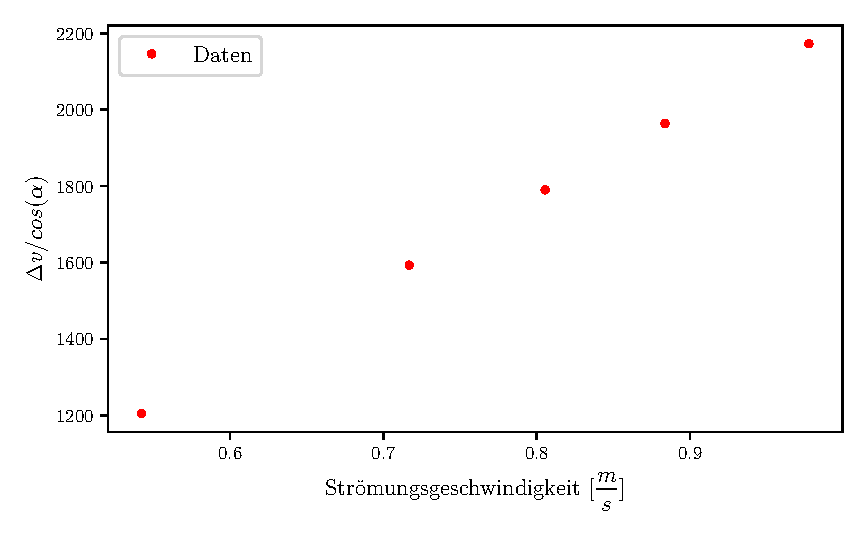
\includegraphics[scale=1]{build/plot1.pdf}
    \caption{Messdaten des Caesiumspektrums.}
    \label{fig:spektrum}
\end{figure}

\begin{table}[H]
    \centering
    \caption{Messergebnisse der Leermessung.}
    \label{tab:0}
    \sisetup{table-format=2.2}
    \begin{tabular}{l S[table-format=2.2] S[table-format=5.0] @{${}\pm{}$} S[table-format=3.0]}
      \toprule
      {Projektion} & {Peak} & \multicolumn{2}{c}{Net Area}\\
      \midrule
        {$I_0$} & 71.60 & 54433 & 255 \\
      \bottomrule
    \end{tabular}
\end{table}



\subsection{Würfel 1}
\label{sub:1}


\begin{table}[H]
  \centering
  \caption{Messergebnisse des ersten Würfels.}
  \label{tab:1}
  \sisetup{table-format=2.2}
  \begin{tabular}{l S[table-format=2.2] S[table-format=5.0] @{${}\pm{}$} S[table-format=3.0]}
    \toprule
    {Projektion} & {Peak} & \multicolumn{2}{c}{Net Area}\\
    \midrule
    $I_2$ & 0 & 52459 & 251 \\ 
    $I_5$ & 0 & 52300 & 249 \\
    \bottomrule
  \end{tabular}
\end{table}

Der Würfel hat eine Wandstärke von $\qty{1}{\milli\meter}$.
Zur Berechnung des Absorptionskoeffizienten von Aluminium wird \autoref{eqn:mu} nach $\mu$ umgestellt.
Da die Wand des Würfels zwei Mal durchstrahlt wird, gilt hier $d=\qty{2}{\milli\meter}$.
Der Mittelwert der Net Area wird nach 
\begin{align*}
  \bar{I}=\frac{1}{n} \sum_{i=1}^n I_i \label{eqn:Mittelwert}
\end{align*}
berechnet zu 
\begin{align*}
  \bar{I}_{\text{Alu}} &=  52379.5.
\end{align*}
Der Fehler berechnet sich analog zu
\begin{align*}
  \Delta \bar{I}_{\text{Alu}} &=  250.0.
\end{align*}

Da mit fehlerbehafteten Größen gerechnet wird ergeben sich die weiteren Fehler mithilfe der Gausschen Fehlerfortpflanzung
\begin{equation*}
  \Delta f=\sqrt{\sum_{j=1}^n \left(\frac{\partial f}{\partial x_j}\Delta x_j \right)^{2}}.\label{eqn:Gauß}
\end{equation*}

$\mu_{\text{Alu}}$ ergibt sich somit zu 
\begin{align*}
  \mu_{\text{Alu}} &= \qty{0.192 \pm 0.527}{\per\centi\meter}
\end{align*}


\subsection{Würfel 2}
\label{sub:2}

Da die weiteren Würfel auch von einer Aluminiumhülle umgeben sind, gilt im Weiteren $I_0 = I_{\text{Alu}}$.
\begin{table}[H]
    \centering
    \caption{Messergebnisse des zweiten Würfels.}
    \label{tab:2}
    \sisetup{table-format=2.2}
    \begin{tabular}{l S[table-format=2.2] S[table-format=5.0] @{${}\pm{}$} S[table-format=3.0]}
      \toprule
      {Projektion} & {Peak} & \multicolumn{2}{c}{Net Area}\\
      \midrule
      $I_1$ & 71.13 & 43944 & 229 \\
      $I_2$ & 71.61 & 44379 & 231 \\
      $I_3$ & 71.59 & 44547 & 231 \\
      $I_4$ & 71.09 & 43508 & 228 \\
      $I_5$ & 71.60 & 43877 & 230 \\
      $I_6$ & 71.59 & 44438 & 231 \\ 
      $I_7$ & 71.58 & 43523 & 227 \\
      $I_8$ & 70.64 & 42419 & 225 \\
      $I_9$ & 71.59 & 45609 & 234 \\ 
      $I_{10}$& 71.63 & 45974 & 235 \\
      $I_{11}$& 70.95 & 42547 & 225 \\
      $I_{12}$& 71.61 & 43347 & 228 \\
      \bottomrule
    \end{tabular}
\end{table}


\begin{table}[H]
  \centering
  \caption{Absorptionskoeffizienten des zweiten Würfels.}
  \label{tab:abs2}
  \sisetup{table-format=1.3}
  \begin{tabular}{l S @{${}\pm{}$} S}
    \toprule
    {Absorptionskoeffizienten} & \multicolumn{2}{c}{Wert in $\si{\per\centi\meter}$}\\
    \midrule
    $\mu_1 $ & 0.053 & 0.005\\
    $\mu_2 $ & 0.077 & 0.003\\
    $\mu_3 $ & 0.047 & 0.005\\
    $\mu_4 $ & 0.062 & 0.003\\
    $\mu_5 $ & 0.045 & 0.004\\
    $\mu_6 $ & 0.057 & 0.003\\
    $\mu_7 $ & 0.060 & 0.005\\
    $\mu_8 $ & 0.039 & 0.003\\
    $\mu_9 $ & 0.057 & 0.005\\
    \bottomrule
  \end{tabular}
\end{table}

Da die Elementarwürfel des zweiten Würfels alle aus einem Material bestehen, wird der Mittelwert aus den berechneten Werten in \autoref{tab:abs2}
gebildet.
Dieser beträgt 
\begin{align*}
  \mu &= qty{0.055 \pm 0.004}{\per\centi\meter}.
\end{align*}


\subsection{Würfel 4}
\label{sub:4}

\begin{table}[H]
    \centering
    \caption{Messergebnisse des vierten Würfels.}
    \label{tab:4}
    \sisetup{table-format=2.2}
    \begin{tabular}{l S[table-format=2.2] S[table-format=5.0] @{${}\pm{}$} S[table-format=3.0]}
      \toprule
      {Projektion} & {Peak} & \multicolumn{2}{c}{Net Area}\\
      \midrule
      $I_1 $ & 71.63 & 41637 & 224 \\
      $I_2 $ & 71.50 & 8834  & 105 \\
      $I_3 $ & 71.70 & 39639 & 217 \\
      $I_4 $ & 71.54 & 14257 & 131 \\
      $I_5 $ & 71.48 & 12719 & 129 \\
      $I_6 $ & 71.47 & 14133 & 131 \\
      $I_7 $ & 71.47 & 8664  & 102 \\
      $I_8 $ & 71.45 & 7798  & 98  \\
      $I_9 $ & 71.49 & 12978 & 124 \\
      $I_{10}$ & 71.44 & 15357 & 136 \\
      $I_{11}$ & 71.46 & 8195  & 99  \\
      $I_{12}$ & 71.44 & 11507 & 118 \\
      \bottomrule
    \end{tabular}
\end{table}


\begin{table}[H]
  \centering
  \caption{Absorptionskoeffizienten des vierten Würfels.}
  \label{tab:abs4}
  \sisetup{table-format=1.3}
  \begin{tabular}{l S @{${}\pm{}$} S c}
    \toprule
    {Absorptionskoeffizienten} & \multicolumn{2}{c}{Wert in $\si{\per\centi\meter}$} & {Material}\\
    \midrule
    $\mu_1 $ & 0.080 & 0.007 & {} \\
    $\mu_2 $ & 0.909 & 0.006 & {} \\
    $\mu_3 $ & 0.087 & 0.007 & {} \\
    $\mu_4 $ & 0.162 & 0.005 & {} \\
    $\mu_5 $ & 0.913 & 0.006 & {} \\
    $\mu_6 $ & 0.175 & 0.005 & {} \\
    $\mu_7 $ & 0.178 & 0.007 & {} \\
    $\mu_8 $ & 0.691 & 0.005 & {} \\
    $\mu_9 $ & 0.211 & 0.007 & {} \\
    \bottomrule
  \end{tabular}
\end{table}
